%% LyX 2.0.0 created this file.  For more info, see http://www.lyx.org/.
%% Do not edit unless you really know what you are doing.
\documentclass[english,traditabstract]{aa}
\usepackage[varg]{txfonts}
%\usepackage[english,brazilian]{babel}
\usepackage[T1]{fontenc}
\setcounter{tocdepth}{3}
\usepackage{prettyref}
\usepackage{array}
\usepackage{rotating}
\usepackage{float}
\usepackage{multirow}
\usepackage{amstext}
\usepackage{graphicx}
\usepackage{epstopdf}
\usepackage{subfigure}
\usepackage{gensymb}
\usepackage{longtable}
\usepackage{color}
%\usepackage{setspace}
%
%\usepackage{etoolbox}
%\AtBeginEnvironment{longtable}{\singlespacing}
%\setlength{\LTcapwidth}{\linewidth}


\makeatletter

%%%%%%%%%%%%%%%%%%%%%%%%%%%%%% LyX specific LaTeX commands.
%% Because html converters don't know tabularnewline
\providecommand{\tabularnewline}{\\}

%%%%%%%%%%%%%%%%%%%%%%%%%%%%%% User specified LaTeX commands.
\usepackage{natbib,twoopt}
\usepackage[breaklinks=true]{hyperref} %% to avoid \citeads line fills
\usepackage{arydshln}
\bibpunct{(}{)}{;}{a}{}{,} %% natbib format for A&A and ApJ
\makeatletter
\newcommandtwoopt{\citeads}[3][][]{\href{http://adsabs.harvard.edu/abs/#3}%
{\def\hyper@linkstart##1##2{}%
\let\hyper@linkend\@empty\citealp[#1][#2]{#3}}}
\newcommandtwoopt{\citepads}[3][][]{\href{http://adsabs.harvard.edu/abs/#3}%
{\def\hyper@linkstart##1##2{}%
\let\hyper@linkend\@empty\citep[#1][#2]{#3}}}
\newcommandtwoopt{\citetads}[3][][]{\href{http://adsabs.harvard.edu/abs/#3}%
{\def\hyper@linkstart##1##2{}%
\let\hyper@linkend\@empty\citet[#1][#2]{#3}}}
\newcommandtwoopt{\citeyearads}[3][][]%
{\href{http://adsabs.harvard.edu/abs/#3}
{\def\hyper@linkstart##1##2{}%
\let\hyper@linkend\@empty\citeyear[#1][#2]{#3}}}
\makeatother
\titlerunning{Predictions of stellar occultations by irregular satellites}
\authorrunning{Gomes-Júnior et al.}

\makeatother


\begin{document}

\title{Predictions of stellar occultations of 9 irregular satellites of giant planets
%\fnmsep\thanks{Table 8 are only available in electronic form at the CDS via anonymous ftp to cdsarc.u-strasbg.fr (130.79.128.5) or via http://cdsweb.u-strasbg.fr/cgi-bin/qcat?J/A+A/ and IAU NSDC data base at www.imcce.fr/nsdc.}
%\fnmsep\thanks{The complete version of Table 8 is available through CDS and IAU NSDC data base at www.imcce.fr/nsdc.}
%\fnmsep\thanks{Partially based on observations made at Laborat\'orio Nacional de Astrof\'{\i}sica (LNA), Itajub\'a-MG, Brazil.}
%\fnmsep\thanks{Partially based on observations through the ESO runs 079.A-9202(A), 075.C-0154, 077.C-0283 and 079.C-0345.}
%\fnmsep\thanks{\textbf{Partially based on observations made at Observatoire de Haute Provence (OHP), F-04870 Saint-Michel l'observatoire, France}}
}

\author{ A. R. Gomes-Júnior
          \inst{1},
          M. Assafin 
          \inst{1} \fnmsep\thanks{Affiliated researcher at Observatoire de Paris/IMCCE, 77 Avenue Denfert Rochereau 75014 Paris, France},
          R. Vieira-Martins
          \inst{1,2,3} \fnmsep\thanks{Affiliated researcher at Observatoire de Paris/IMCCE, 77 Avenue Denfert Rochereau 75014 Paris, France},
%          J.-E. Arlot
%          \inst{4},      
          J. I. B. Camargo
          \inst{2,3},     
%          F. Braga-Ribas
%          \inst{2,4}, 
%          D. N. da Silva Neto
%          \inst{6},
%          A. H. Andrei
%          \inst{1,2} \fnmsep\thanks{Affiliated researcher at Observatoire de Paris/SYRTE, 77 Avenue Denfert Rochereau, 75014 Paris, France},
          B. E. Morgado
          \inst{1},
%          A. Dias-Oliveira
%          \inst{2},
%          G. Benedetti-Rossi
%          \inst{2},
%          Y. Duchemin
%          \inst{4,7},
%          J. Desmars
%          \inst{4},
%          V. Lainey
%          \inst{4},
%          W. Thuillot
%          \inst{4}
          }

\offprints{A. R. Gomes-Júnior}

   \institute{Observatório do Valongo/UFRJ, Ladeira Pedro Antônio 43,
CEP 20.080-090 Rio de Janeiro - RJ, Brazil\\
              \email{altair08@astro.ufrj.br}
              \and
Observatório Nacional/MCT, R. General José Cristino 77,
CEP 20921-400 Rio de Janeiro - RJ, Brazil\\
              \email{rvm@on.br}
              \and
Laboratório Interinstitucional de e-Astronomia - LIneA, Rua Gal. José Cristino 77, Rio de Janeiro, RJ 20921-400, Brazil
%              \and
%Institut de mécanique céleste et de calcul des éphémérides - Observatoire %de Paris, UMR 8028 du CNRS,
%77 Av. Denfert-Rochereau, 75014 Paris, France\\
%              \email{arlot@imcce.fr}
%              \and
%Federal University of Technology - Paraná (UTFPR / DAFIS), Rua Sete de Setembro, 3165, CEP 80230-901, Curitiba, PR, Brazil
%              \and
%Centro Universitário Estadual da Zona Oeste, Av. Manual Caldeira de Alvarenga 1203, CEP 23.070-200 Rio de Janeiro RJ, Brazil
%              \and
%              ESIGELEC-IRSEEM, Technopôle du Madrillet, Avenue Galilée, 76801 Saint-Etienne du Rouvray, France
              }



\date{Received ; accepted }


\abstract
%{The irregular satellites of the giant planets are believed to have been captured during the evolution of the solar system. Knowing their physical parameters, such as size, density and albedo is important to constrain where they came from and how they were captured. The best way to obtain these parameters are observations in situ by spacecrafts or from stellar occultations by the objects. Both techniques demand that the orbits are well known.}
%{We aimed to obtain good astrometric positions of irregular satellites in order to improve their orbits and ephemeris.}
%{We identified and reduced observations of several irregular satellites from three databases containing more than 8000 images obtained between 1992 and 2014 at three sites (Observatório do Pico dos Dias, Observatoire de Haute-Provence and European Southern Observatory - La Silla).  We used the software PRAIA (Platform for Reduction of Astronomical Images Automatically) to make the astrometric reduction of the CCD frames. The UCAC4 catalogue represented the International Celestial Reference System in the reductions. The identification of the satellites in the frames was done through their ephemerides as determined from the SPICE/NAIF kernels. Some procedures were taken to overcome missing or incomplete information (coordinates, date), mostly for the older images.}
%{We managed to obtain more than 6000 positions for 18 irregular satellites, being 12 of Jupiter, 4 of Saturn, 1 of Uranus (Sycorax) and 1 of Neptune (Nereid). For some satellites the number of obtained positions is more than 50\% of that used in earlier orbital numerical integrations.}
%{Comparison of our positions with recent JPL ephemeris suggests the presence of systematic errors in the orbits for some of the irregular satellites. The most evident case was an error in the inclination of Carme.}


\keywords{Occultations - Planets and satellites: general - Planets and satellites: individual: Jovian and Saturnian irregular satellites}

\maketitle

\section{Introduction} \label{Sec: introducao} 

Irregular satellites, also known as outer satellites, of the giant planets are objects orbiting the planets from a distant, eccentric and highly inclined orbit, most of them are retrograde. Because of these peculiar orbits, it is largely accepted that these objects were captured by their planets in the early solar system \citep{Sheppard2005}.

There is a number of capture mechanisms of objects by giant planets proposed in the literature. There is the Gas Drag in the primordial circumplanetary nebulae \citep{Sheppard2005} where the object would be affected by the gas drag and its velocity slowed down until it be captured by the planet. Another mechanism is called pull-down capture \citep{Sheppard2005}, where the mass of the planet would increase while the object was temporarily captured. 

A mechanism based in the Nice model \citep{Morbidelli2005, Tsiganis2005, Gomes2005} was proposed by \cite{Nesvorny2007} and, in the specific case of Jupiter with the modern Nice model, by \citealp{Nesvorny2014}. During the early solar system instability, encounters between the outer planets occurred. These planetary encounters could exchange energy and angular momentum between planets and the objects nearby making it possible for the capture of irregular bodies by the giant planets. In this scenario, the survival rate of prior-LHB (Late Heavy Bombardment) satellites is very small.

Another important mechanism is the capture through collisional interactions \citep{Sheppard2005}. A collision between two small bodies in the Hill's sphere of the planet could generate fragmented objects and the dissipated energy could be such that some of these objects could be captured.

Some of these objects are in dynamical groups with similar orbital elements, called families, similar to families found in the Main Asteroid Belt. These families may have been created by a parent body disrupted by collisions with comets or other satellites \citep{Nesvorny2004}. Collisions with comets are more likely to have occurred during the Late Heavy Bombardment (LHB) \citep{Gomes2005}.

\cite{Nesvorny2003} studied the collision rates between irregular satellites and concluded that some satellites could have been removed by collision with a bigger satellite. The rate collision between satellites of the Himalia Group (Himalia, Elara, Lysithea and Leda, mainly), for instance, was found to be more than one during the solar system age suggesting that their current structure was originated by satellite-satellite collision.

For Phoebe, ejected material from its surface caused by impacts could evolve due to Poynting-Robertson drag and collide with Iapetus causing the large variation in albedo observed on it \citep{Nesvorny2003}. Indeed, Cassini was able to detected in Phoebe an absorption feature at 2.42 $\mu m$ (probably CN combinations) that was also detected in the dark side of Iapetus \citep{Clark2005}.

The region of origin of these object is not well known, \cite{Grav2003} and \cite{Grav2007} showed that the irregular satellites from the giant planest have their colors and spectral slopes similar to C-, D- and P-type asteroids, Centaurs and trans-neptunian objects (TNOs) suggesting that they have been originated from different locations in the early solar system.

In this work, we study these objects as possible representatives of the small TNOs population. TNOs are objects that due to their distance may be highly preserved having their properties similar to those they had when they were formed, then providing history and evolution of the outer solar system \citep{Camargo2013}. Due to their distance, the smaller objects from this region are more difficult to observe and study.

In the intent to obtain the physical parameters (size, shape, albedo, density, etc) of the irregular satellites and help identify their origin locations, we will make use of the stellar occultation technique. This technique is the best one to obtain these parameters of the solar system objects from ground-based observations providing more accurate results than other ground-based techniques \citep{Sicardy2011, Ortiz2012, Braga-Ribas2014}.

Since their estimated sizes are very small (see table \ref{} \textcolor{red}{Ainda vou fazer a tabela}), predict the exact location and instant where the shadow will cross the Earth demands a good precision. For instance, the bigger irregular satellite of Jupiter has an estimated size of 150 km \citep{Porco2003}, which is equivalent to an apparent size of 40 mas, must have an error smaller than its size for being observable. For the other objects, smaller or farther than Himalia, the situation is more difficult.

As pointed out by \cite{GomesJunior2015}, the ephemeris of the irregular satellites have errors that may reach 200 mas for some satellites. For an object at the distance of Jupiter, this represents an error bigger than 700 km in the shadow path.

We present in this paper the stellar occultation predictions for the 7 major irregular satellites of Jupiter (Himalia, Elara, Pasiphae, Lysithea, Carme, Ananke and Sinope), Phoebe from Saturn and Triton and Nereid from Neptune. In the section \ref{Sec: Rationale} we explore the scientific rationale for study the irregular satellites and the possibility of having a common origin with TNOs. In section \ref{Sec: Offset} we show the correction made to the ephemeris for better predict stellar occultations. In section \ref{Sec: predictions}, we present the predictions of the stellar occultations by irregular satellites and how they were made. Some test realized to confirm the predictions are presented in section \ref{Sec: testes} and the conclusion is given in section \ref{Sec: conclusions}.

\section{Scientific Rationale} \label{Sec: Rationale}

As explicited in section \ref{Sec: introducao}, there is no consensus on a single model about the region where the irregular satellites were formed. In this work we treat them as having a common origin to the Centaurs and TNOs. In this case, they would be the representative objects of the small TNOs population. Since that small objects at great distances are difficult to study, the irregular satellites can complement this gap.

%This idea is supported by the 

%Because they are faint, the majority of these objects was discovered only in the last century\footnote{Website: http://ssd.jpl.nasa.gov/?sat\_discovery} . They were never visited by a spacecraft, with the exception of Himalia, Phoebe and Nereid, in a flyby by the Cassini space probe in 2000 for Himalia \citep{Porco2003} and in 2004 for Phoebe \citep{Desmars2013} and in a flyby by the Voyager 2 space probe in 1989 for Nereid \citep{Smith1989}. Even in situ, they were still opportunity target observations resulting in not optimal measurements, with size errors of $10 km$ for Himalia and $25 km$ for Nereid \citep{Thomas1991}. The exception is Phoebe with a very accurate measurement of size with a mean radius error of $0.7 km$ \citep{Thomas2010}.

%If these objects were captured, there remains the question of where they came from. \citealp{Clark2005} showed from imaging spectroscopy from Cassini that Phoebe has a surface probably covered by material from the outer solar system and \citealp{Grav2003} showed that the satellites of the Jovian Prograde Group Himalia have grey colors implying that their surfaces are similar to that of C-type asteroids. In that same work, the Jovian Retrograde Group Carme was found to have surface colors similar to the D-type asteroids like Hilda or Trojan families while JXIII Kalyke has a redder color like Centaurs or trans-neptunian objects (TNOs).

%For Saturnian satellites, \citealp{Grav2007} showed by their colors and spectral slopes that these satellites contain a more or less equal fraction of C-, P- and D-like objects but SXXII Ijiraq is marginally redder than D-type objects. These works may suggest different origins for the irregular satellites.

%In this context, we used 3 databases for deriving precise positions for the irregular satellites observed at Observatório do Pico dos Dias (1.6 m and 0.6 m telescopes, IAU code 874), Observatoire Haute-Provence (1.2m telescope, IAU code 511) and ESO (2.2 m telescope, IAU code 809). Many irregular satellites were observed between 1992 and 2014 covering a few orbital periods of these objects (12 satellites of Jupiter, 4 of Saturn, Sycorax of Uranus and Nereid of Neptune). 

%Since their ephemerides are not very precise, predict and observe stellar occultations are very difficult and no observation of such an event for an irregular satellite is found in the literature. The precise star positions to be derived by the ESA astrometry satellite Gaia \citep{deBruijne2012} will render better predictions with the only source of error being the ephemeris. The positions derived from \textbf{our} observations can be used in new orbital numerical integrations, generating more precise ephemerides.

%The power of stellar occultations for observing relatively small diameter solar system objects is supported by recent works such as the discovery of a ring system around the Centaur (10199) Chariklo \citep{Braga-Ribas2014}. Once irregular satellites start to be observed by this technique, it will be possible to obtain their physical parameters (shape, size, albedo, density) with unprecedented precision. For instance, in this case, sizes could be obtained with kilometer accuracy. The knowledge of these parameters would in turn bring valuable information for the study of the capture mechanisms and origin of the irregular satellites.

%The databases are described in Sect. \ref{Sec: observations}. The astrometric procedures in Sect. \ref{Sec: reduction}. The obtained positions are presented in Sect \ref{Sec: positions} and analysed in Sect. \ref{Sec: comparison}. Conclusions are given in Sect. \ref{Sec: conclusions}.

\section{Correction of the ephemeris} \label{Sec: Offset}

\cite{GomesJunior2015} showed from observations made at the Observatório do Pico dos Dias (OPD), Observatoire Haute-Provence (OHP) and European Southern Observatory (ESO) that the orbits of the irregular satellites of the giant planets have systematic errors. The offsets of the observations relative to the JPL ephemeris could be up to 200 mas for some satellites. These differences could be associated with errors in their orbital elements.

Making a new model for the orbits of these objects would demand a lot of time and delay the publication of these predictions. Then we utilize the offsets obtained by \cite{GomesJunior2015} to identify a pattern in the error of the ephemeris. This pattern could be used to extrapolate an offset to the satellite ephemeris by the time of the occultation predicted. Plots of the offsets over time and true anomaly (see Fig. \ref{Fig:offxtime} and \ref{Fig:offxtanom} for Carme) clearly show the systematic error in the JPL ephemeris.

\begin{figure}
\begin{centering}
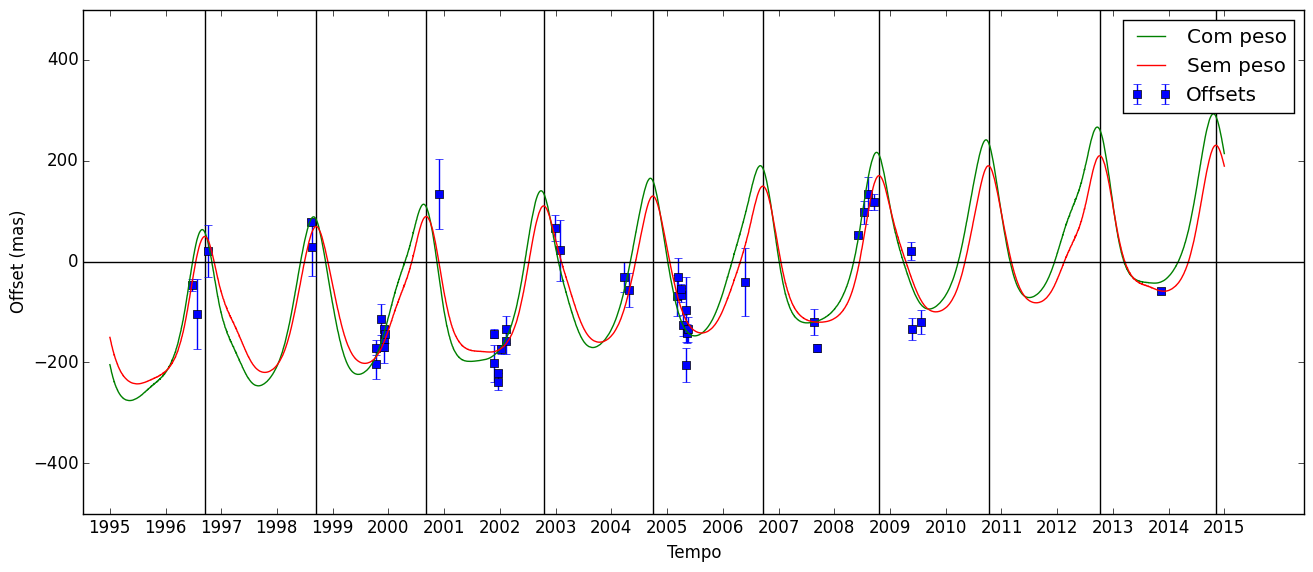
\includegraphics[scale=0.25]{figures/DEC.png}\label{Fig:offxtime}
\caption{Offsets of the declination of Carme by time. \textcolor{red}{Figura só para visualização, vou colocar alguma melhor depois}}
\end{centering}
\end{figure}

\begin{figure}
\begin{centering}
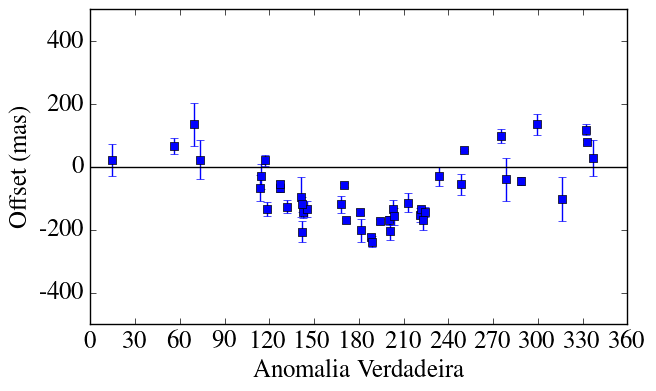
\includegraphics[scale=0.25]{figures/DEC_anom.png} \label{Fig:offxtanom}
\caption{Offsets of the declination of Carme by true anomaly. \textcolor{red}{Figura só para visualização, vou colocar alguma melhor depois}}
\end{centering}
\end{figure}



\begin{equation}
F(t,f) = p[0]\times t + p[1]\times \sin(f) + p[2]\times\cos(f) + p[3],
\label{eq:linear}
\end{equation}

\begin{equation}
\begin{split}
%F = \{F_{x} \in  F_{c} &: (|S| > |C|) \\
% &\quad \cap (\text{minPixels}  < |S| < \text{maxPixels}) \\
% &\quad \cap (|S_{\text{conected}}| > |S| - \epsilon) \}
F(t,f) = p[0]\times\sin\left(\frac{2\pi}{p[1]}\times t + p[2]\right) + p[3]\times\sin(f) + \\ +p[4]\times\cos(f) + p[5],
\end{split}
\end{equation}
where $F(t,f)$ is the offset obtained, $t$ is time in years counting from J2000.0 and $f$ is the true anomaly.

\textcolor{red}{Falta justificar as funções}



\section{Prediction of occultations} \label{Sec: predictions}

The prediction of the occultations was made by crossing the stellar coordinates and proper motions of the UCAC4 catalogue \citep{Zacharias2013} with the corrected JPL ephemeris as presented in the section \ref{Sec: Offset}. The search for stellar candidates follows the same procedure as presented by \cite{Assafin2010, Assafin2012} and \cite{Camargo2013}.

It was predicted occultation by the 7 major irregular satellites of Jupiter, Phoebe of Saturn and Triton and Nereid of Neptune.

For Triton and Nereid, the candidates for stellar occultations in 2015 and 2016 was searched using the WFI catalogue in the same way as the predictions for Centaurs and TNOs occultations by \cite{Assafin2010, Assafin2012} and \cite{Camargo2013}. This catalogue contains the stars in the path of Neptune in the sky up to mid-2016. The catalogue was generated by observations made at the ESO 2p2 telescope (IAU code 809) using the Wide Field Imager (WFI) CCD mosaic detector. The filter used was the broad-band R filter ESO\#844 with $\lambda_c$ = 651.725 nm and $\Delta\lambda$ = 162.184 nm.

A total of 588 events \textcolor{red}{(Não estou contando ainda os eventos para Tritão)} were identified between January 2015 and December 2017. Table \ref{Tab: occ-list} exemplifies the catalogue of occultations generated and their parameters, which is necessary to produce occultation maps (see Fig. \ref{Fig: ocultacao} as an example). Since these objects are very small, the duration of each event is a few seconds.

\begin{table*}
\caption{\label{Tab: sample-cds} Extract of prediction table. \textcolor{red}{Ainda tenho que fazer a tabela melhor, encaixar. Abaixo é um exemplo apenas para visualização.}}
\begin{centering}
\begin{tabular}{ccccccccccccccccccccccc}
\hline 
%\multicolumn{9}{c}{Himalia} \tabularnewline
\hline
% & \multicolumn{2}{c}{Mean errors} & Nr & Nr &  UCAC4       \tabularnewline
d m Year & h m s & \multicolumn{2}{c}{RA (ICRS) Dec} & C/A & P/A & v & D & R* & $\lambda$ & LST & $\Delta e_{\alpha *}$ & $\Delta e_{\delta}$ & pm & ct & $E_{\alpha *}$ & $E_{\delta}$ & $\mu_{\alpha *}$ & $\mu_{\delta}$ \tabularnewline
\hline
 07 10 2015 & 21 52 34. &  10 53 40.1835 & +08 21  00.489 & 0.465 & 200.31 & 39.31 & 6.25 & 16.6 & 179. & 09:48 & -31.0 & -13.0 & ok & uc &   0  &  0 & -13 &  -7 \tabularnewline
 23 10 2015 & 07 54 50. &  11 05 26.6037 & +07 14  32.030 & 1.017 & 201.33  & 36.11 & 6.12 & 15.5 & 16. & 08:59 & -31.0 & -13.0 & ok & uc &  0  &  0 &  -7 &  -4 \tabularnewline
%\texttt{ d  m year  h:m:s UT     ra\_\_\_dec\_\_\_J2000\_candidate     ra\_dec\_J2000\_target\_geocen     C/A    P/A     vel  Delta  R*   J*   H*   K*   long  loc. t.  off\_ra   off\_de pm ct f E\_ra E\_de pmra pmde} \tabularnewline
%\hline
% 05 01 2015  01 07  4.   09 32 20.9233 +15 35  10.584   09 32 20.9885 +15 35  12.220   1.888   29.94 -11.41  4.51 14.8 -0.6 -0.6 -0.6    22. 02:35     -31.0    -13.0 ok uc 0    0    0   -4    1 \tabularnewline
% 15 01 2015  01 03 15.   09 29  0.9265 +16 01  18.932   09 29  0.9610 +16 01  19.900   1.088   27.21 -13.17  4.45 14.8 -0.5 -0.5 -0.5    12. 01:52     -31.0    -13.0 ok uc 0    0    0   -2  -16 \tabularnewline
% 02 02 2015  08 03 30.   09 21 46.5321 +16 49  43.658   09 21 46.4857 +16 49  42.068   1.723  202.72 -14.32  4.40 16.0 -0.4 -0.4 -0.4   247. 00:32     -31.0    -13.0 ok uc 0    0    0    1   -8 \tabularnewline
% 14 02 2015  16 11 59.   09 16 41.4840 +17 18   2.448   09 16 41.4473 +17 18   0.976   1.563  199.68 -13.64  4.42 12.5 -0.4 -0.4 -0.4   112. 23:39     -31.0    -13.0 ok uc 0    0    0    5    0 \tabularnewline
% 25 02 2015  19 27 38.   09 12 25.6457 +17 38   6.563   09 12 25.6804 +17 38   8.217   1.727   16.72 -12.01  4.47 12.2 -0.6 -0.6 -0.6    51. 22:51     -31.0    -13.0 ok uc 0    0    0   -3    4 \tabularnewline
% 28 02 2015  09 17 38.   09 11 31.5455 +17 41  53.701   09 11 31.5720 +17 41  55.023   1.375   15.96 -11.50  4.49 14.1 -0.6 -0.6 -0.6   201. 22:40     -31.0    -13.0 ok uc 0    0    0  -16    6 \tabularnewline
% 03 03 2015  00 39 17.   09 10 38.6352 +17 45  26.467   09 10 38.6218 +17 45  25.758   0.734  195.15 -10.94  4.50 14.1 -0.7 -0.7 -0.7   327. 22:28     -31.0    -13.0 ok uc 0    0    0   -5    2 \tabularnewline
% 20 05 2015  08 59 41.   09 13 37.6521 +16 48  39.598   09 13 37.6915 +16 48  41.011   1.522   21.84  17.60  5.48 15.2 -0.1 -0.1 -0.1   126. 17:22     -31.0    -13.0 ok uc 0    0    0    0    0 \tabularnewline
% 22 05 2015  06 52 27.   09 14 25.8437 +16 44   5.646   09 14 25.8400 +16 44   5.511   0.147  201.62  18.32  5.51 16.4 -0.1 -0.1 -0.1   156. 17:16     -31.0    -13.0 ok uc 0    0    0  -13    2 \tabularnewline
% 02 06 2015  16 14 18.   09 19 46.8676 +16 14  30.501   09 19 46.8693 +16 14  30.569   0.078   20.53  22.38  5.67 14.5  0.1  0.1  0.1     6. 16:36     -31.0    -13.0 ok uc 0    0    0   -7  -15 \tabularnewline
% 06 06 2015  02 41  6.   09 21 34.2809 +16 04  53.249   09 21 34.2951 +16 04  53.800   0.588   20.32  23.54  5.71 16.4  0.2  0.2  0.2   206. 16:24     -31.0    -13.0 ok uc 0    0    0    2    5 \tabularnewline
% 08 06 2015  20 25 31.   09 23  3.2029 +15 57   1.059   09 23  3.2057 +15 57   1.170   0.122   20.13  24.44  5.75 16.7  0.2  0.2  0.2   297. 16:15     -31.0    -13.0 ok uc 0    0    0   -3   -6 \tabularnewline
% 09 06 2015  22 29 56.   09 23 39.2777 +15 53  51.969   09 23 39.2451 +15 53  50.681   1.372  200.09  24.80  5.76 11.6  0.2  0.2  0.2   265. 16:11     -31.0    -13.0 ok uc 0    0    0    5  -24 \tabularnewline
% 20 06 2015  16 15 15.   09 29 57.6850 +15 21   0.007   09 29 57.7127 +15 21   1.135   1.198   19.56  28.11  5.90 16.4  0.4  0.4  0.4   350. 15:35     -31.0    -13.0 ok uc 0    0    0   -8   -1 \tabularnewline
% 05 07 2015  17 02 21.   09 39 45.6144 +14 31  18.362   09 39 45.6473 +14 31  19.747   1.465   19.04  32.07  6.06 16.7  0.5  0.5  0.5   326. 14:46     -31.0    -13.0 ok uc 0    0    0    0   -9 \tabularnewline
% 16 07 2015  03 15 38.   09 47  5.8941 +13 54  48.764   09 47  5.8853 +13 54  48.387   0.400  198.77  34.42  6.15 16.4  0.6  0.6  0.6   164. 14:12     -31.0    -13.0 ok uc 0    0    0  -19  -10 \tabularnewline
% 07 10 2015  21 52 34.   10 53 40.1835 +08 21   0.489   10 53 40.1726 +08 21   0.054   0.465  200.31  39.31  6.25 16.6  0.7  0.7  0.7   179. 09:48     -31.0    -13.0 ok uc 0    0    0  -13   -7 \tabularnewline
% 23 10 2015  07 54 50.   11 05 26.6037 +07 14  32.030   11 05 26.5789 +07 14  31.083   1.017  201.33  36.11  6.12 15.5  0.6  0.6  0.6    16. 08:59     -31.0    -13.0 ok uc 0    0    0   -7   -4 \tabularnewline
% 31 10 2015  00 24 19.   11 10 56.2964 +06 42   7.110   11 10 56.3414 +06 42   8.782   1.801   21.84  33.94  6.04 16.9  0.6  0.6  0.6   123. 08:34     -31.0    -13.0 ok uc 0    0    0   -4  -13 \tabularnewline
% 07 11 2015  21 22 53.   11 16 14.3041 +06 10   5.194   11 16 14.2963 +06 10   4.912   0.306  202.36  31.33  5.94 16.2  0.5  0.5  0.5   162. 08:09     -31.0    -13.0 ok uc 0    0    0    0    0 \tabularnewline
% 08 11 2015  04 27 21.   11 16 25.7881 +06 08  55.566   11 16 25.7606 +06 08  54.571   1.077  202.38  31.23  5.94 16.9  0.5  0.5  0.5    55. 08:08     -31.0    -13.0 ok uc 0    0    0    9  -10 \tabularnewline
% 09 11 2015  09 01  4.   11 17 11.6890 +06 04  11.474   11 17 11.7030 +06 04  11.980   0.549   22.45  30.79  5.92 15.9  0.5  0.5  0.5   346. 08:04     -31.0    -13.0 ok uc 0    0    0   19  -13 \tabularnewline
% 11 11 2015  12 58 46.   11 18 33.8286 +05 55  43.695   11 18 33.8357 +05 55  43.946   0.274   22.59  29.98  5.90 14.6  0.4  0.4  0.4   285. 07:57     -31.0    -13.0 ok uc 0    0    0  -14    1 \tabularnewline
% 12 11 2015  20 14 22.   11 19 22.2740 +05 50  40.732   11 19 22.3183 +05 50  42.312   1.713   22.68  29.48  5.88 15.7  0.4  0.4  0.4   175. 07:52     -31.0    -13.0 ok uc 0    0    0   -7   -4 \tabularnewline
% 04 12 2015  03 31 56.   11 30 41.9967 +04 37  36.039   11 30 42.0020 +04 37  36.217   0.196   24.18  20.14  5.56 15.0  0.0  0.0  0.0    47. 06:40     -31.0    -13.0 ok uc 0    0    0    5   -9 \tabularnewline

% 31 10 2015  00 24 19.   11 10 56.2964 +06 42   7.110   11 10 56.3414 +06 42   8.782   1.801   21.84  33.94  6.04 16.9  0.6  0.6  0.6   123. 08:34     -31.0    -13.0 ok uc 0    0    0   -4  -13 \tabularnewline
% 07 11 2015  21 22 53.   11 16 14.3041 +06 10   5.194   11 16 14.2963 +06 10   4.912   0.306  202.36  31.33  5.94 16.2  0.5  0.5  0.5   162. 08:09     -31.0    -13.0 ok uc 0    0    0    0    0 \tabularnewline
% 08 11 2015  04 27 21.   11 16 25.7881 +06 08  55.566   11 16 25.7606 +06 08  54.571   1.077  202.38  31.23  5.94 16.9  0.5  0.5  0.5    55. 08:08     -31.0    -13.0 ok uc 0    0    0    9  -10 \tabularnewline
% 09 11 2015  09 01  4.   11 17 11.6890 +06 04  11.474   11 17 11.7030 +06 04  11.980   0.549   22.45  30.79  5.92 15.9  0.5  0.5  0.5   346. 08:04     -31.0    -13.0 ok uc 0    0    0   19  -13 \tabularnewline
% 11 11 2015  12 58 46.   11 18 33.8286 +05 55  43.695   11 18 33.8357 +05 55  43.946   0.274   22.59  29.98  5.90 14.6  0.4  0.4  0.4   285. 07:57     -31.0    -13.0 ok uc 0    0    0  -14    1 \tabularnewline
% 12 11 2015  20 14 22.   11 19 22.2740 +05 50  40.732   11 19 22.3183 +05 50  42.312   1.713   22.68  29.48  5.88 15.7  0.4  0.4  0.4   175. 07:52     -31.0    -13.0 ok uc 0    0    0   -7   -4 \tabularnewline
% 04 12 2015  03 31 56.   11 30 41.9967 +04 37  36.039   11 30 42.0020 +04 37  36.217   0.196   24.18  20.14  5.56 15.0  0.0  0.0  0.0    47. 06:40     -31.0    -13.0 ok uc 0    0    0    5   -9 \tabularnewline
\hline
\end{tabular}
\par\end{centering}
\textbf{Notes}. Occultation table: day of the year and UTC time of the prediction; right ascension and declination of the occulted star - in the original table, these coordinates are immediately followed by the geocentric astrometric equatorial coordinates (corrected for the offset or ephemeris method), not presented here, of the occulting body; C/A: the geocentric closest approach, in arcseconds; P/A: the planet position angle with respect to the occulted star at C/A, in degrees; velocity in plane of sky, in km s$^{-1}$: positive = prograde, negative = retrograde; D: planet range to Earth, in AU; R*, J*, H*, K*: normalized magnitudes to a common shadow velocity of 20 km s$^{-1}$ by the relationship $\textrm{Mag}* = \textrm{Mag}_{\textrm{actual}} + 2.5 \times \log 10 \left(\frac{\textrm{velocity}} {20 \textrm{km}\, \textrm{s}^{-1}} \right)$. A value of 50.0 means that the star is not in the 2MASS; $\lambda$: east longitude of subplanet point in degrees, positive towards east; LST: UT + $\lambda$: local solar time at subplanet point, hh:mm; $\Delta e_{\alpha *}$ and $\Delta e_{\delta}$:offset in mas applied to the ephemeris right ascension and declination, respectively; pm: ok = proper motion applied, no = no proper motion applied; catalogue cross-identification (ct) = uc (UCAC2), 2m (2MASS), fs (field star); f = multiplicity flag (see Table 3); $E_{\alpha *}$ and $E_{\delta}$: uncertainties (mas) in right ascension and declination. A value of 9999 means that there was no estimation of the respective uncertainty; $\mu_{\alpha *}$ and $\mu_{\delta}$: proper motions in right ascension and declination, respectively (mas/year).
\label{Tab: occ-list}
\end{table*}

\begin{figure}
\begin{centering}
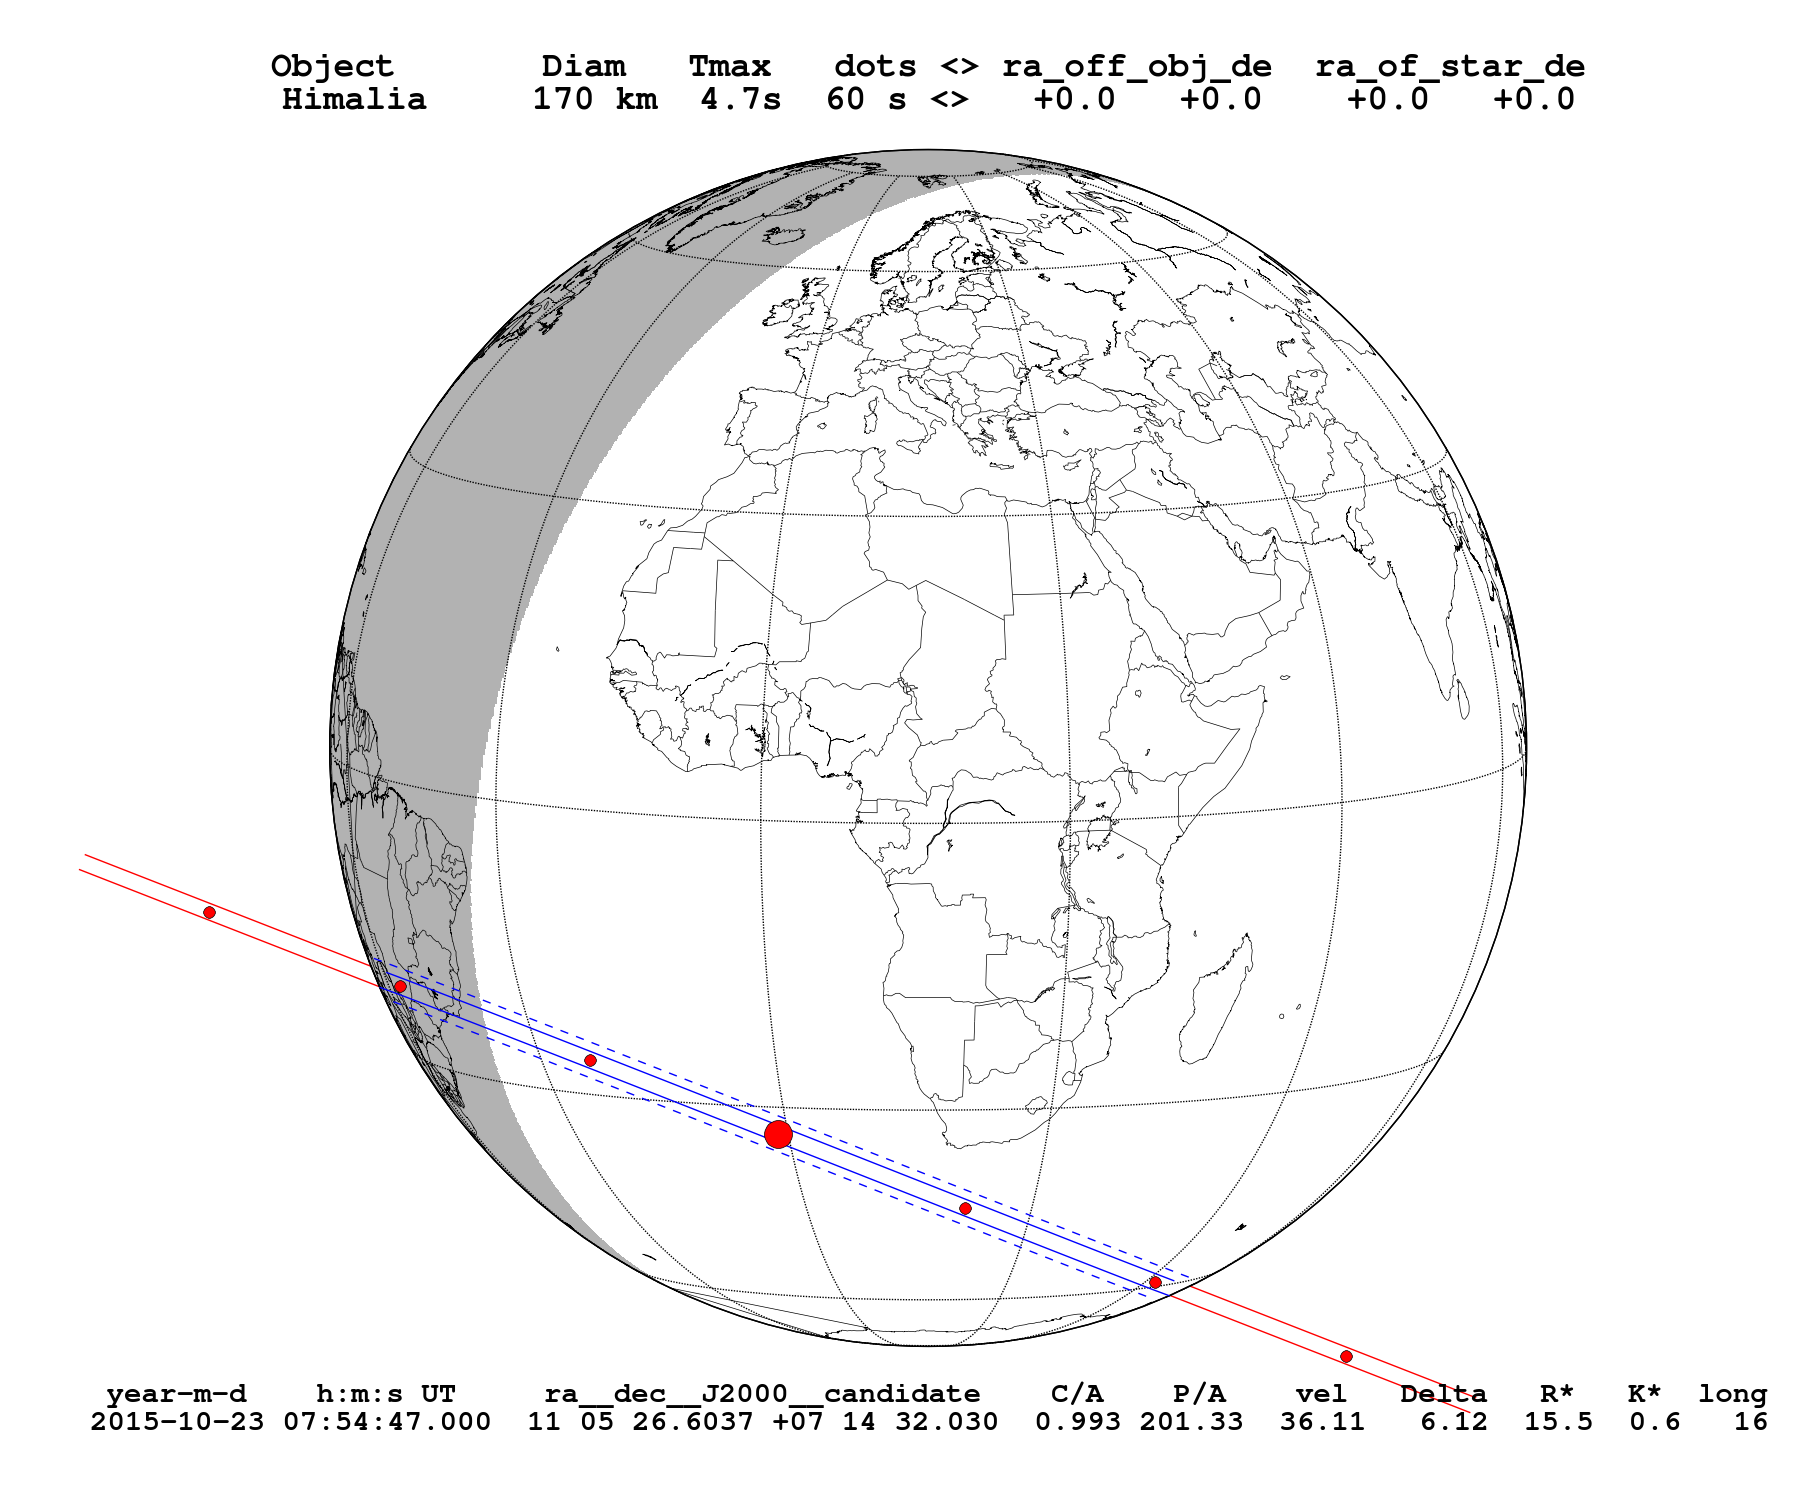
\includegraphics[scale=0.2]{figures/Himalia_2015-10-23T07:54:47.png} 
\caption{Occultation map for Himalia \textcolor{red}{Mapa de Himalia para exemplificar, posso colocar outro depois}. Compare the information given in caption with the second entry of Table \ref{Tab: occ-list}}
\label{Fig: ocultacao}
\end{centering}
\end{figure}


\section{Occultation tests} \label{Sec: testes}

Observe a stellar occultation by an irregular satellites demands a great effort. The shadow covers a very restricted area on Earth because the irregular satellites are small. So before we start a large observational campaign, we tested some occultation predictions for larger objects, to assess the quality of the prediction.

This test consists in observing the object and star to be occulted near the event when the two objects are present in the same field of view, preferably when the objects are close to each other. Thus the relative positions between the two objects will have minimal influence of the errors of the catalogue of stars used and possible field distortions.

To date, two occultation tests were performed, one by Himalia that occurred on March 3, 2015 and the second by Elara that occurred on March 30, 2015. For each event, four maps were generated: the first with the nominal positions of the star and the satellite to the predicted time; the second with the offset calculated as described in section \ref{Sec: Offset}; the third with star and satellite offsets from observations made a few days before the occultation when the two objects were separated (different FOV); and the fourth from observations made when the star and the satellite were close in the same FOV.

Figure \ref{Fig: occ-Himalia}. Shows the four maps for Himalia occultation test in March 03, 2015. The map \ref{Fig: occ-Himalia-nooff} is the nominal prediction with the coordinate of the star given by the catalogue and that of the satellite from the ephemeris. We then corrected the positions of the satellite by an offset calculated by the method showed in section \ref{Sec: Offset} to make the map \ref{Fig: occ-Himalia-ajuste}.

The map \ref{Fig: occ-Himalia-off22fev} was made from obtained positions on February 22 observed with the Zeiss telescope at the Observatório do Pico dos Dias (OPD). On that day, Himalia and the star were observed in separate FOVs as they were still far apart. On the night of the event, March 3, the objects were observed with Perkin-Elmer telescope at OPD just over an hour after the time scheduled for the event. Satellite and star were separated by about 16 arcsec, so very close to each other. From the calculated offsets, the map \ref{Fig: occ-Himalia-off03mar} was generated.

\begin{figure*}
\begin{centering}
\subfigure[Nominal prediction]{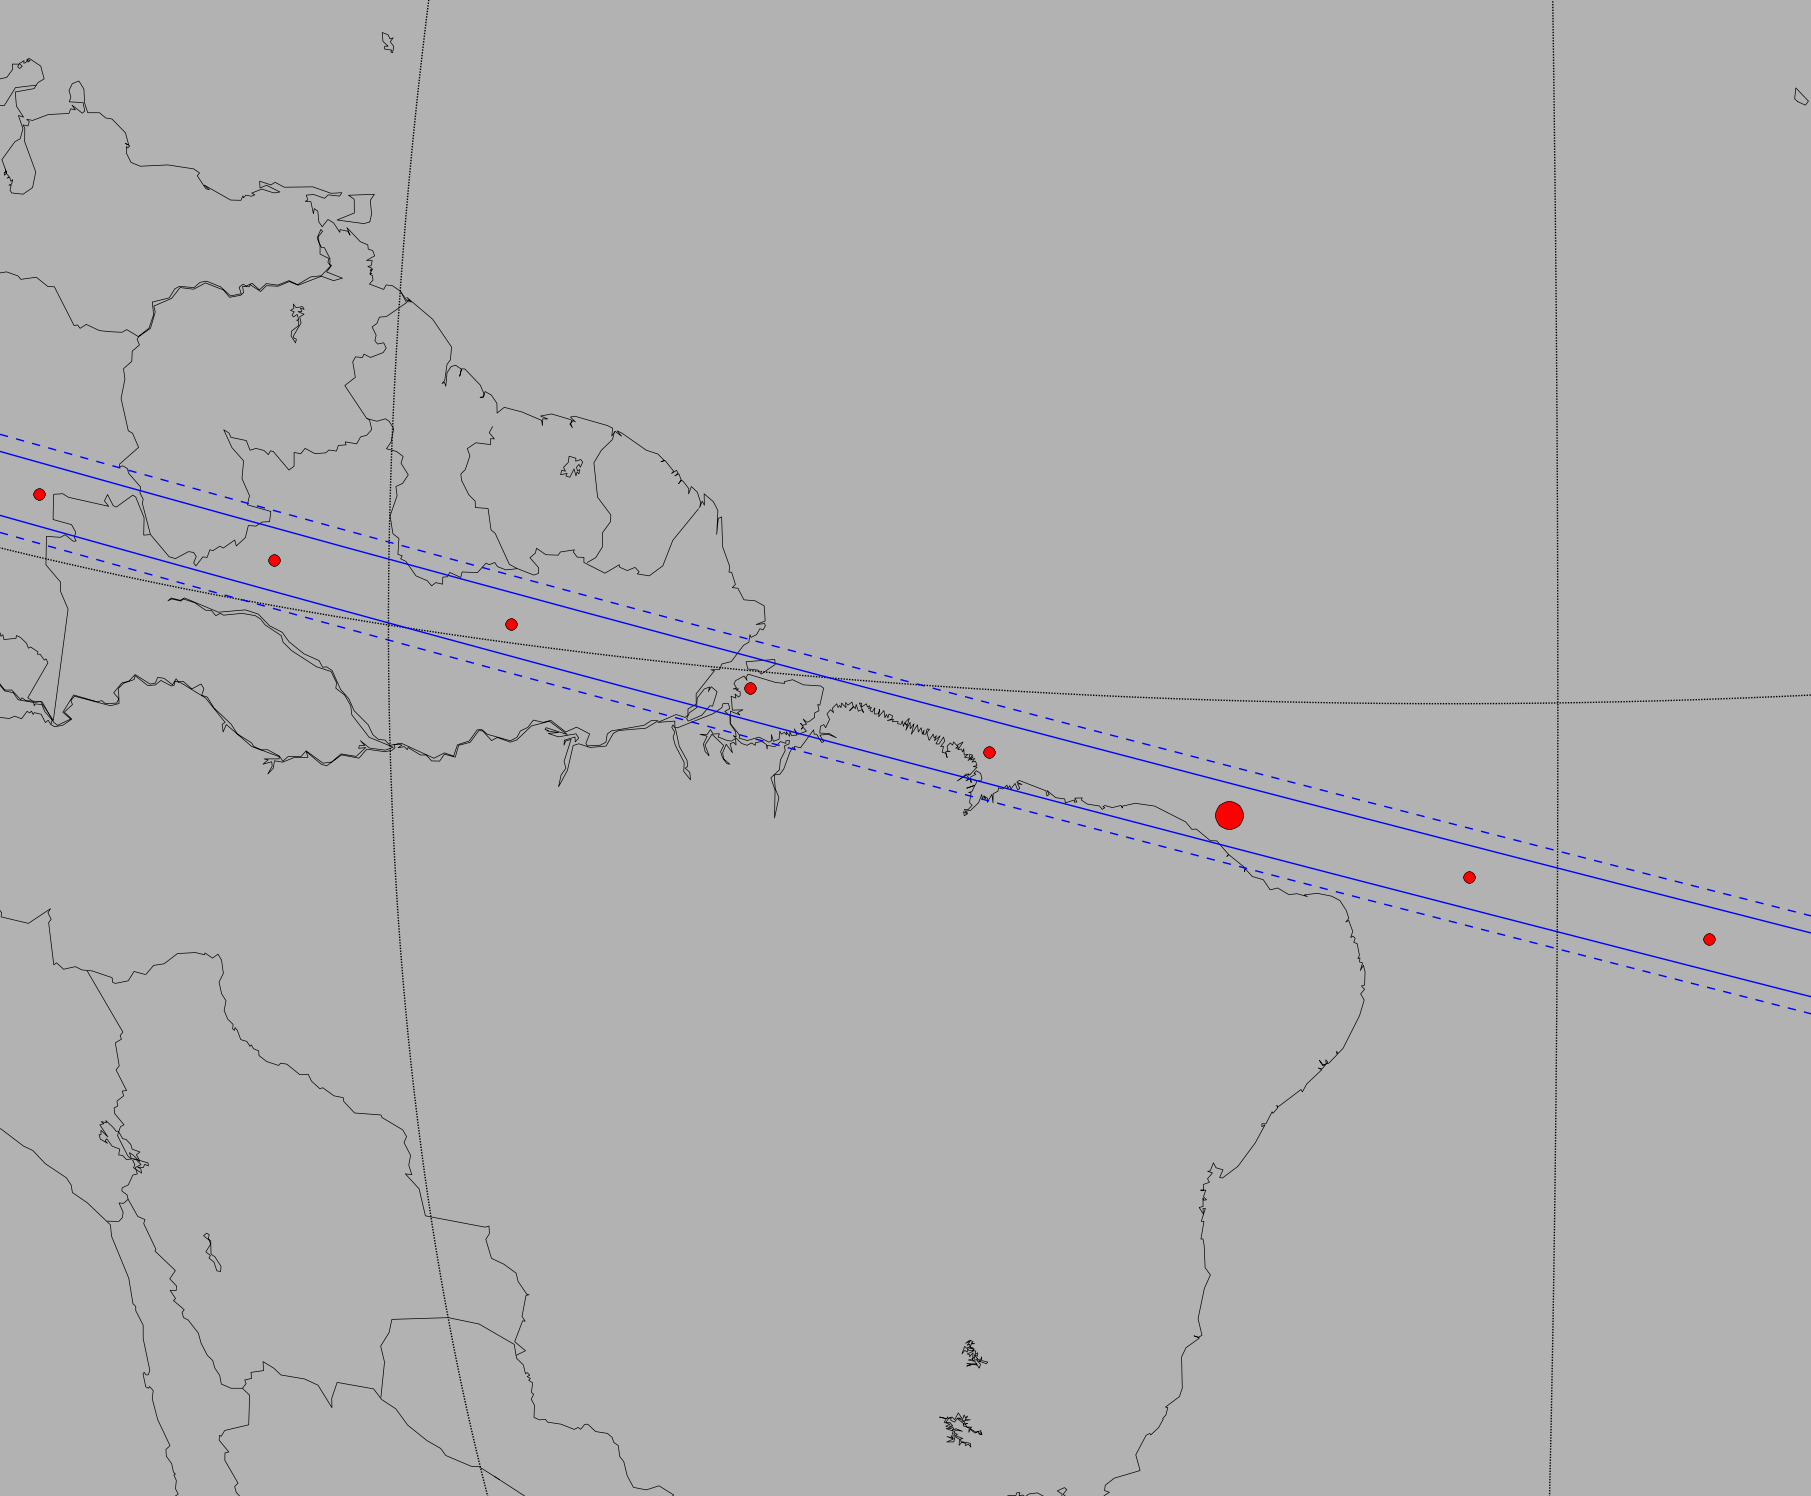
\includegraphics[scale=0.19]{figures/Himalia1_2015-03-03T00:39:25.png}  \label{Fig: occ-Himalia-nooff}}
\subfigure[\textcolor{red}{Offset de Himalia a partir do ajuste}]{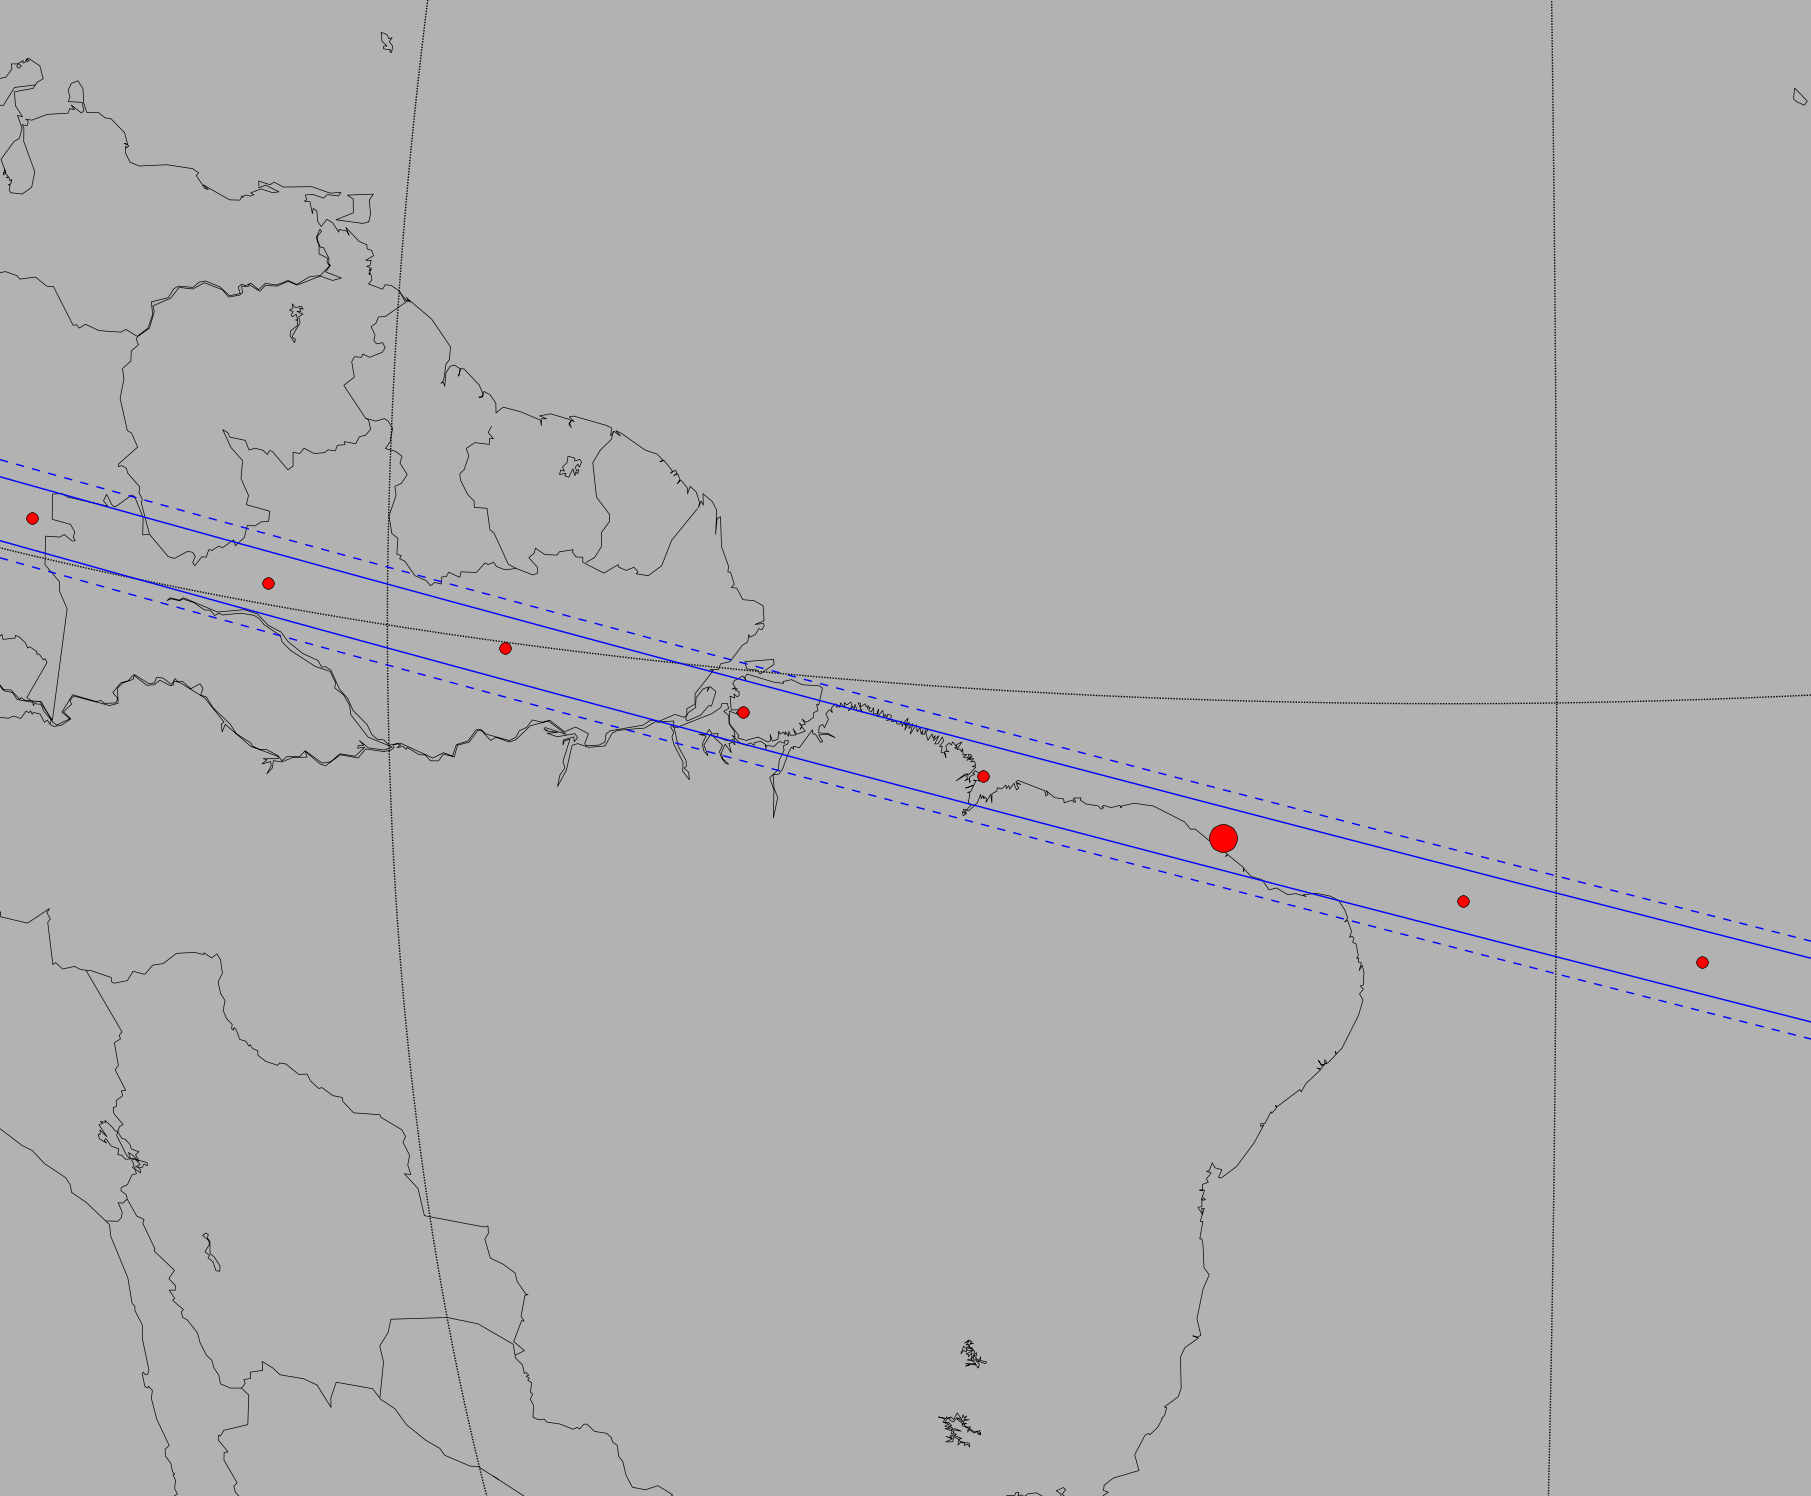
\includegraphics[scale=0.19]{figures/Himalia2_2015-03-03T00:39:18.png}  \label{Fig: occ-Himalia-ajuste}}
\subfigure[February 22 observations (different FOVs)]{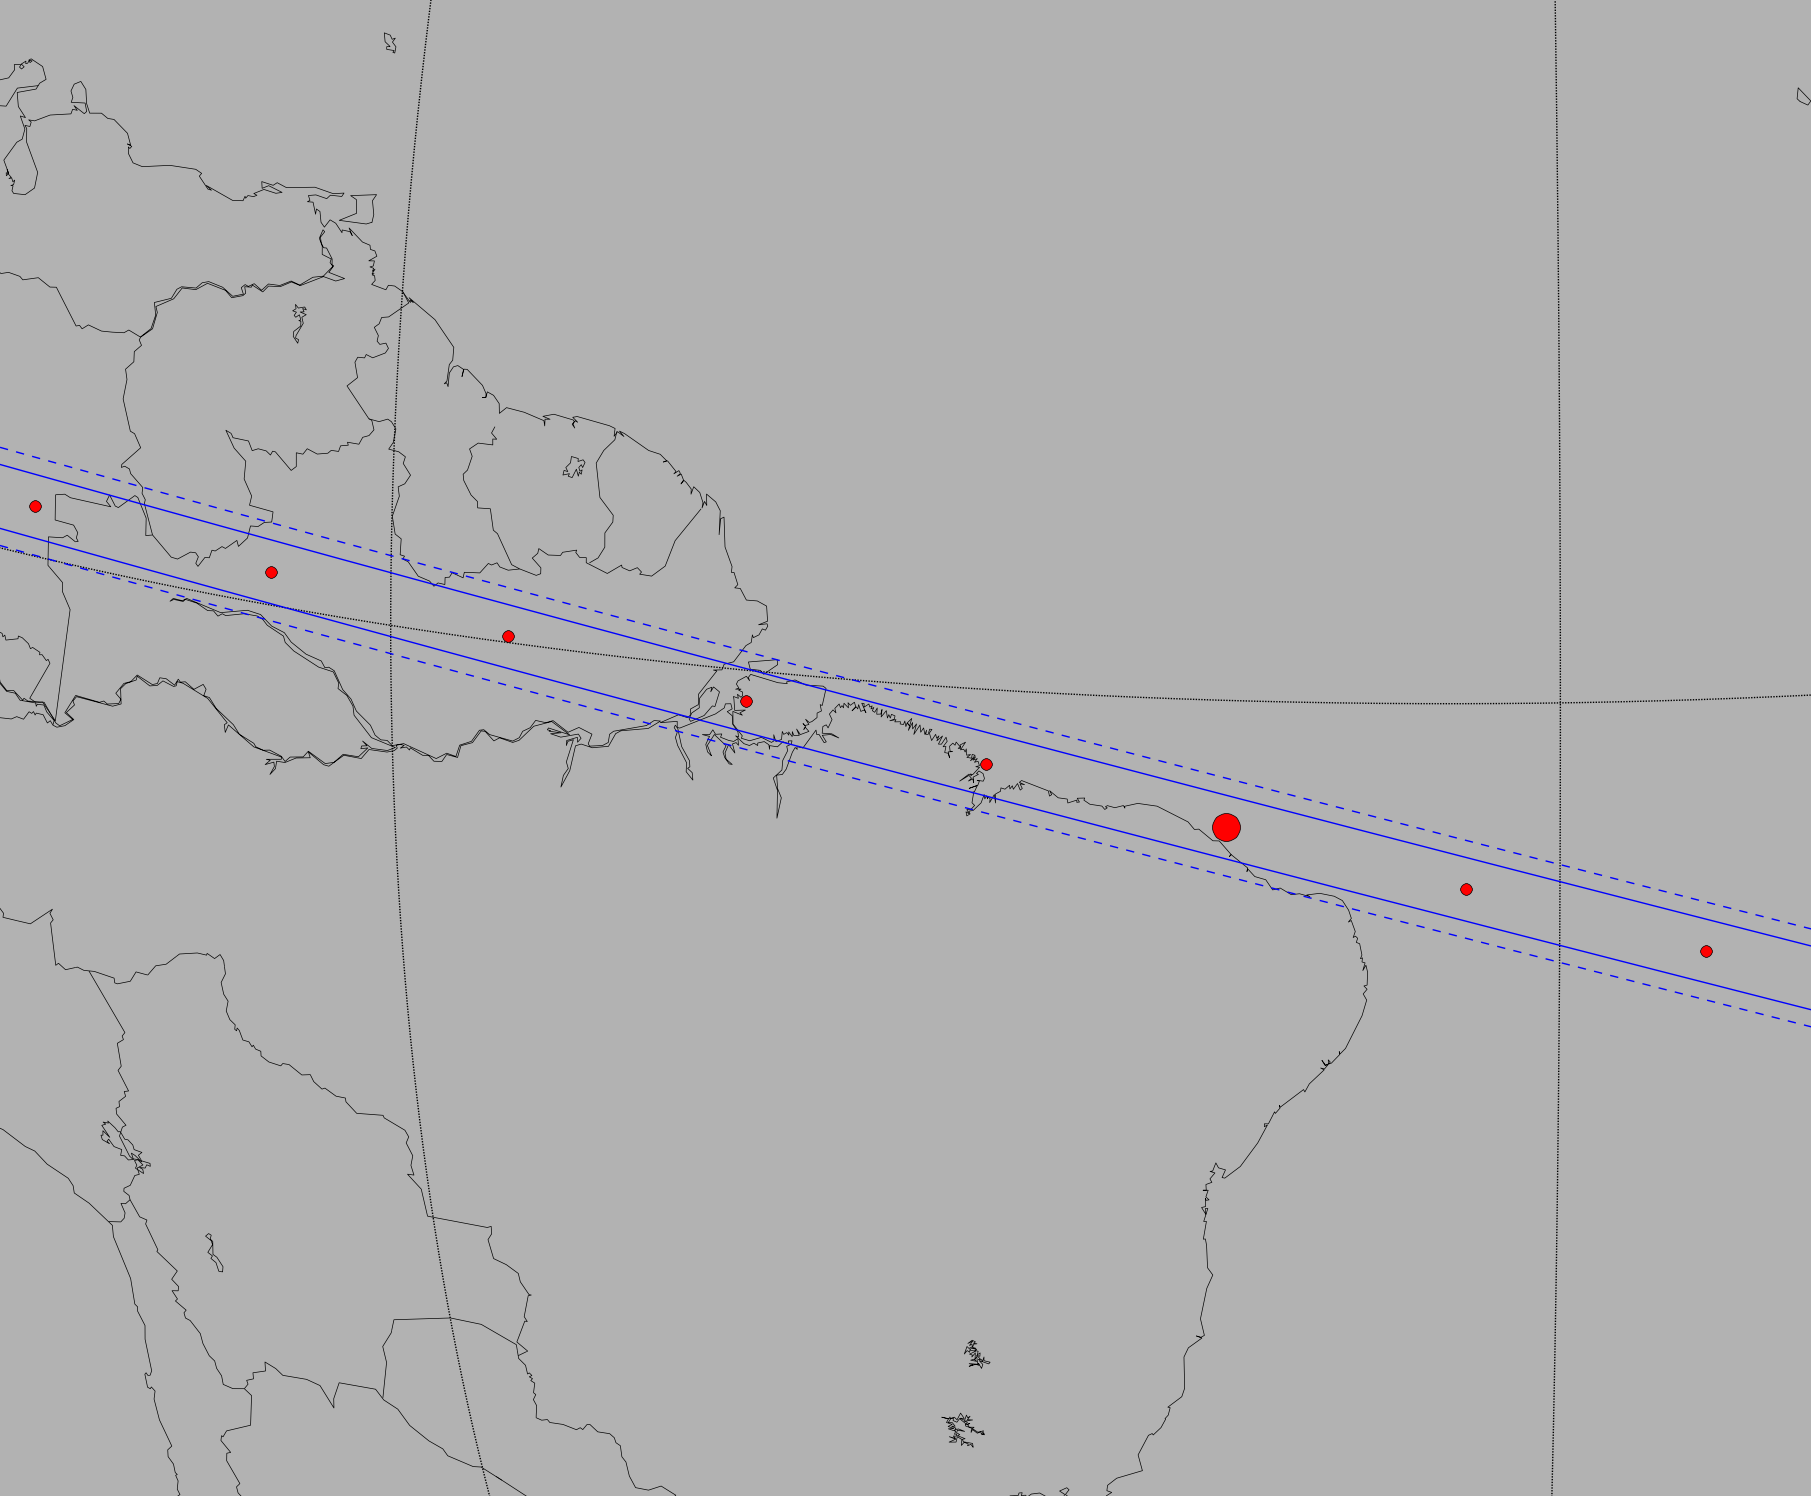
\includegraphics[scale=0.19]{figures/Himalia3_2015-03-03T00:39:40.png}   \label{Fig: occ-Himalia-off22fev}}
\subfigure[March 03 observation (same FOV)]{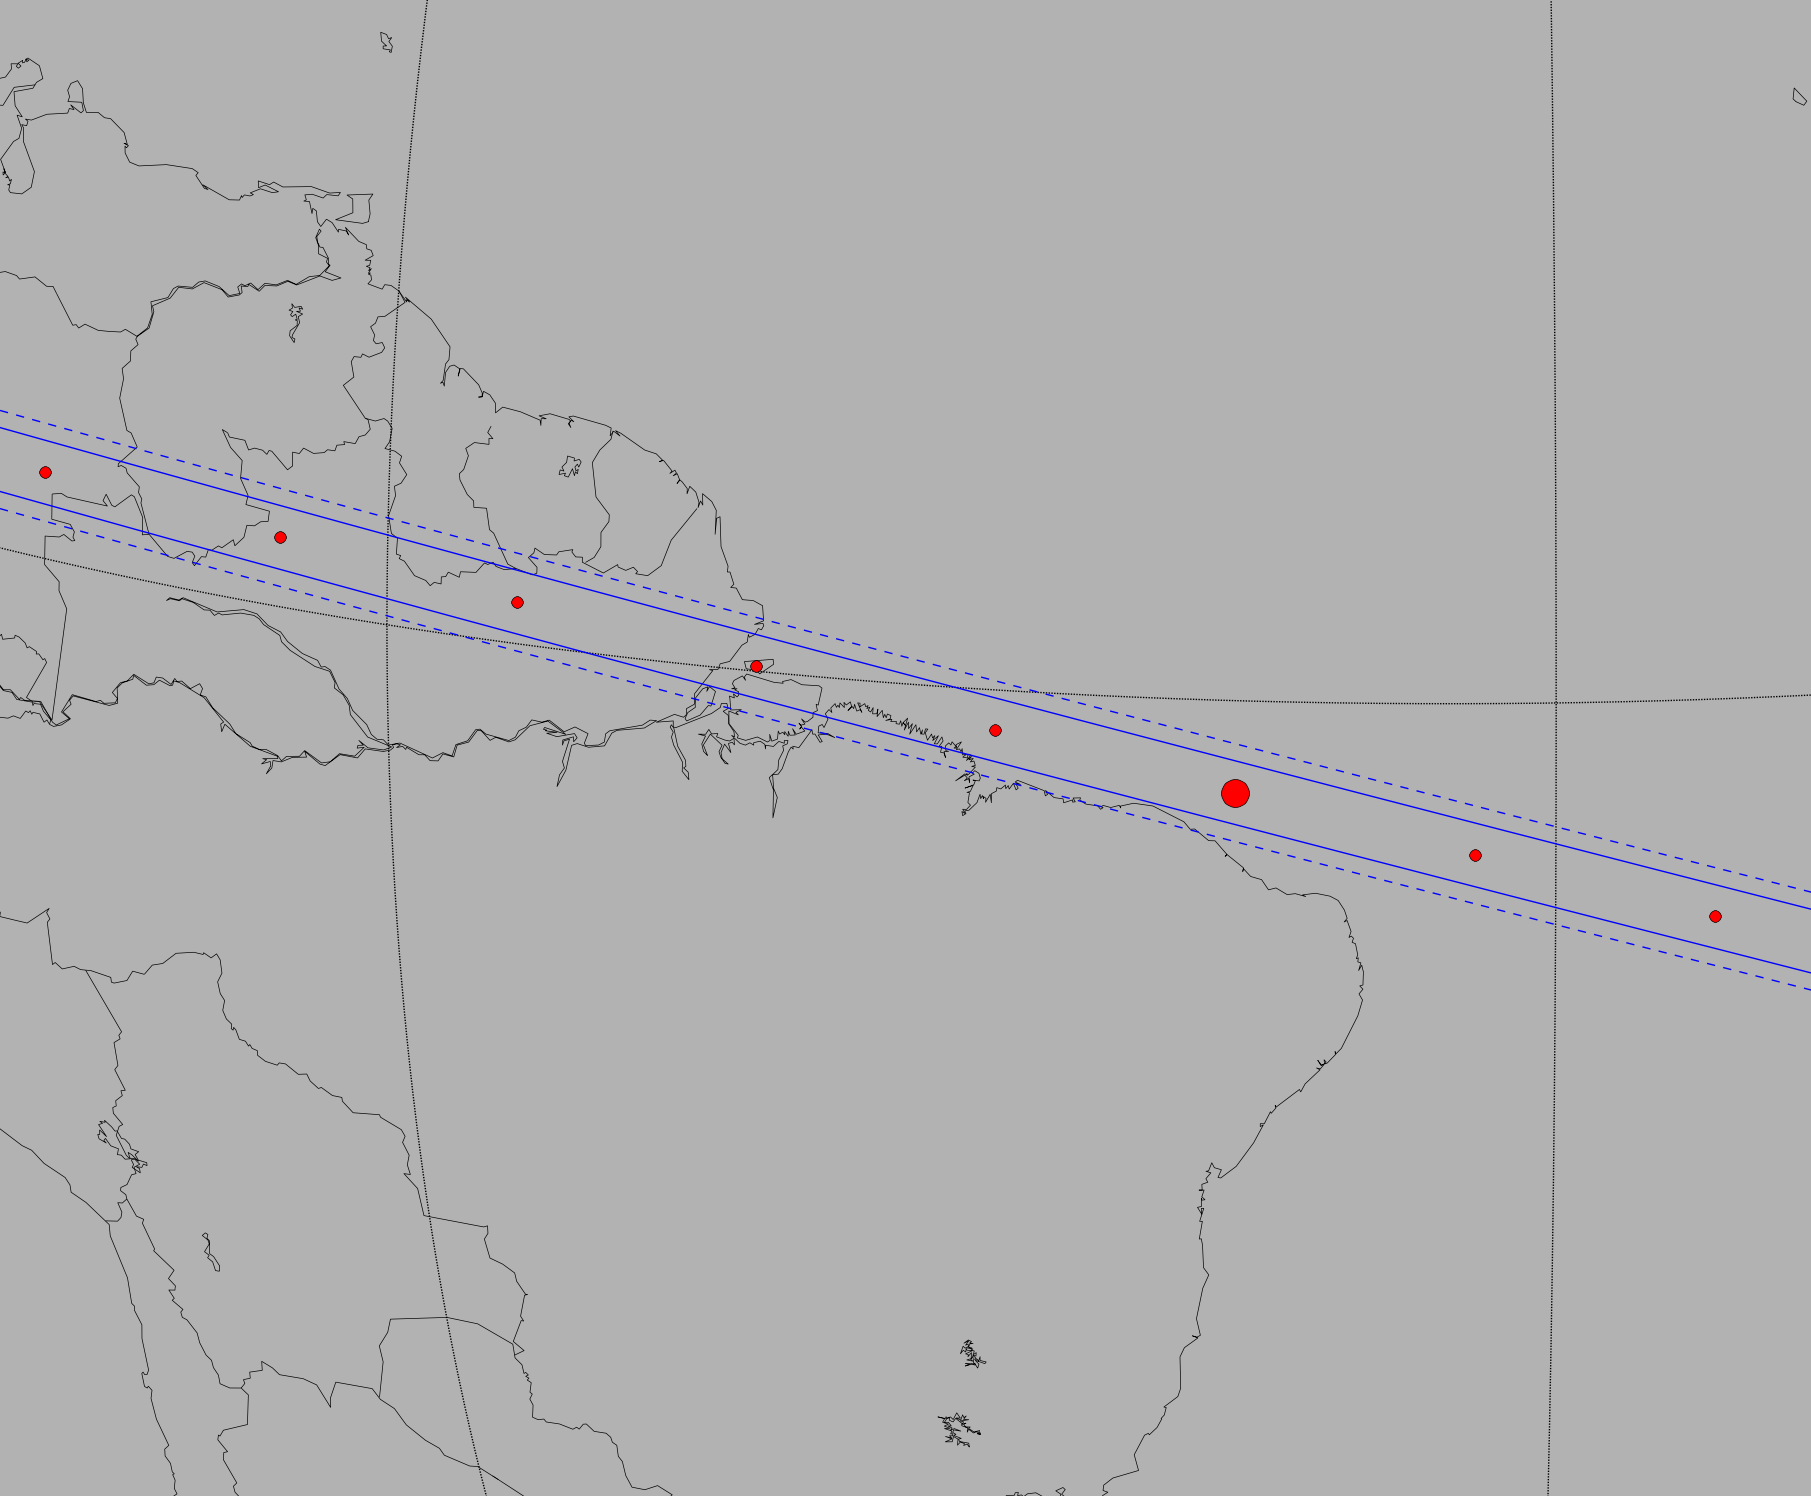
\includegraphics[scale=0.19]{figures/Himalia4_2015-03-03T00:39:15.png}   \label{Fig: occ-Himalia-off03mar}}
\caption{Predictions for Himalia: The big red dot show the geocentric closest approach of the shadow. The small red ones are the center of the shadow separated by one minute. The straight lines show the size of the shadow. \ref{Fig: occ-Himalia-nooff} is the map using the nominal positions of the star and satellite. \ref{Fig: occ-Himalia-ajuste} shows the shadow given an estimated offset for the position of Himalia related to the JPL ephemeris obtained in section \ref{Sec: Offset}. In \ref{Fig: occ-Himalia-off22fev} we apply offsets to the positions of star and satellite accordingly the observations made at February 22. In \ref{Fig: occ-Himalia-off03mar} is as in \ref{Fig: occ-Himalia-off22fev} but with observations made at March 03 when the objects were close to each other. \textcolor{red}{Figuras ainda serão mudadas. Colocadas para visualização}}
\label{Fig: occ-Himalia}
\end{centering}
\end{figure*}

In this event, it is possible to see that the shade does not vary much among the four maps suggesting that, at least for Himalia, there is a greater probability of observing an event. In fact, the biggest difference between the shadows of the four maps are 25s and 130km in the direction perpendicular to the shadows (see table \ref{Tab: comparison-Himalia}).

\begin{table}
\caption{\label{Tab: comparison-Himalia} Comparison between the predictions of Himalia. \textcolor{red}{Ainda vou terminar de preencher a tabela e tem que ver direito o offset do ajuste}}
\begin{centering}
\begin{tabular}{lcc}
\hline  \hline
\multicolumn{3}{c}{Difference from nominal prediction} \tabularnewline
Method  & Instant of C/A  & C/A   \tabularnewline
\hline
Nominal & 2015-03-03 00:39:25 UT & $0.714\arcsec$ \tabularnewline
Offset & -07 s & \tabularnewline
Feb. 22 Obs. & +15 s &  \tabularnewline
Mar. 03 Obs. & -10 s & \tabularnewline
\hline
\end{tabular}
\par\end{centering}
\end{table}

The second test was with the satellite Elara, which is the second biggest irregular satellites of Jupiter. The event was predict the occur at March 30, 2015. The observations were taken on March 25 and April 2, 2015 with the Zeiss telescope. On the night of April 2 they could still be observed in the same FOV. Due to Elara be much weaker, dispersions of the satellite positions on both nights ended up being higher than for Himalia. Still, the differences between the maps obtained were relatively small. The biggest difference between them is 73s and 302km (see table \ref{Tab: comparison-Elara}).

\begin{table}
\caption{\label{Tab: comparison-Elara} Comparison between the predictions of Elara. \textcolor{red}{Ainda vou terminar de preencher a tabela e tem que ver direito o offset do ajuste}}
\begin{centering}
\begin{tabular}{lcc}
\hline  \hline
\multicolumn{3}{c}{Difference from nominal prediction} \tabularnewline
Method  & Instant of C/A  & C/A  \tabularnewline
\hline
Nominal & 2015-03-30 01:45:15 UT & $1.139\arcsec$ \tabularnewline
Offset & -16 s & \tabularnewline
Mar. 25 Obs. & -58 s &  \tabularnewline
Apr. 02 Obs. & +15 s & \tabularnewline
\hline
\end{tabular}
\par\end{centering}
\end{table}


\section{Conclusion} \label{Sec: conclusions}

%We managed a large database with FITS images acquired by 5 telescopes in 3 sites between 1992 and 2014. From that, we identified 8466 observations of irregular satellites, from which we managed to obtain 6523 suitable astrometric positions, giving a total of 3666 positions for 12 satellites of Jupiter, 1920 positions for 4 satellites of Saturn, 35 positions for Sycorax (Uranus) and 902 positions for Nereid (Neptune).

%The positions of all the objects were determined using the PRAIA package. The package was suited to cope with the huge amount of observations and the task of identifying the satellites within the database. PRAIA tasks were also useful to deal with the missing or incorrect coordinate and time stamps present mostly in the old observations.The UCAC4 was used as the reference frame. Based in the comparisons with ephemeris, we estimate that the position errors are about 60 mas to 80 mas depending on the satellite brightness.

%For some satellites the number of positions obtained in this work is comparable to the number used in the numerical integration of orbits by the JPL \citep{Jacobson2012} (see Table \ref{Tab: comparison-horizons}). For instance, the amount of new positions for Himalia is about 70\% of the number used in the numerical integation of orbits by JPL. Systematic errors in the ephemeris were found for at least some satellites (Ananke, Carme, Elara and Pasiphae). In the case of Carme, we evidenced an error in the orbital inclination (see Fig. \ref{Fig: carme_anom}).

%The positions derived in this work can be used in new orbital numerical integrations, generating more precise ephemerides. Stellar occultations by irregular satellites could then be better predicted. Based in this work, our group has already computed occultation predictions for the 8 major irregular satellites of Jupiter. These predictions will be published in a forthcoming paper.


\begin{acknowledgements}

ARG-J thanks the financial support of CAPES. MA thanks the CNPq (Grants 473002/2013-2 and 308721/2011-0) and FAPERJ (Grant E-26/111.488/2013). RV-M thanks grants: CNPq-306885/2013, Capes/Cofecub-2506/2015, Faperj/PAPDRJ-45/2013. JIBC acknowledges CNPq for a PQ2 fellowship (process number 308489/2013-6). FB-R acknowledges PAPDRJ-FAPERJ/CAPES E-43/2013 number 144997, E-26/101.375/2014. BEM thanks the financial support of CAPES.

\end{acknowledgements}

\bibliographystyle{aa}
\nocite{*}
\bibliography{references.bib}


\end{document}
